% -----------------------------*- LaTeX -*------------------------------
\documentclass[UTF8]{report}
% ------------------------------------------------------------------------
% Packages
% ------------------------------------------------------------------------
\usepackage{ctex} % 支持中文
\usepackage[body={7in, 9in},left=1in,right=1in]{geometry} % 改变页边距
\usepackage{amsmath} % AMS 的数学宏包
\usepackage{amsfonts} % AMS 的数学字体宏包
\usepackage{amssymb} % AMS 符号库
\usepackage{bm} % 数学公式中的黑斜体h
\usepackage{amsthm} % AMS 的定理环境宏包
\usepackage{graphicx} % 插图
\usepackage{subfigure} % 插子图
\usepackage{nicefrac} % 好看的分数
\usepackage{mathrsfs} % mathscr font
\usepackage{caption} % caption
\usepackage{algorithm,algorithmicx} % 伪代码支持宏包
\usepackage[noend]{algpseudocode} % 伪代码
\usepackage{fancyhdr} % 设置页眉、页脚
\usepackage{adjustbox} % 图片尺寸自动调整
\usepackage{esint} % 积分符号
\usepackage{mathtools} % 数学宏包的重要补充
\usepackage{upgreek} % 数学环境的直立希腊字母
\usepackage{enumitem} % 使用enumitem宏包, 改变列表项的格式
\usepackage{color} % 支持彩色
\usepackage{extarrows} % 任意长度的箭头
\usepackage{tikz} % 绘图
\usepackage{forest} % 绘树
\usepackage{xcolor} % 颜色宏包
\usepackage{breqn} % 公式自动换行
\usepackage{fontsize} % 字体大小
\usepackage[framemethod=TikZ]{mdframed} % 给文字加框
\usepackage{fontspec} % 字体库
\usepackage{bigstrut} % 用于表格中的换行
\usepackage{multirow} % 表格中多行单元格合并
\usepackage{multicol} % 表格中多列单元格合并
\usepackage{longtable} % 长表格
\usepackage{rotating} % 旋转图形和表格      以上三者用于绘制三线表
\usepackage{booktabs} % 三线表宏包
\usepackage{scribe} % Scribe 模板
\usepackage{diagbox} % 表格斜线
\usepackage{listings} % 插入代码
\usepackage{verbatim} % 多行注释
\usepackage{ifplatform} % 检测编译平台
\usepackage{hyperref} % 超链接
\usepackage{mathrsfs} % 花体
\usepackage{pgffor} % foreach
\usepackage{circuitikz} % 画电路图
\usepackage{svg} % 插入svg
\usetikzlibrary{shapes.geometric, arrows} % 引入流程图需要的库
\usetikzlibrary{automata} % 引入automata库
\usetikzlibrary{shapes,arrows,positioning,chains} % 引入positioning库
% ------------------------------------------------------------------------
% Macros
% ------------------------------------------------------------------------
%~~~~~~~~~~~~~~~
% Utility latin
%~~~~~~~~~~~~~~~
\newcommand{\ie}{\textit{i.e.}}
\newcommand{\eg}{\textit{e.g.}}
%~~~~~~~~~~~~~~~
% Environment shortcuts
%~~~~~~~~~~~~~~~
\newcommand{\balign}[1]{\ealign{\begin{align}#1\end{align}}}
\newcommand{\baligns}[1]{\ealigns{\begin{align*}#1\end{align*}}}
\newcommand{\bitemize}[1]{\eitemize{\begin{itemize}#1\end{itemize}}}
\newcommand{\benumerate}[1]{\eenumerate{\begin{enumerate}#1\end{enumerate}}}
%~~~~~~~~~~~~~~~
% Text with quads around it
%~~~~~~~~~~~~~~~
\newcommand{\qtext}[1]{\quad\text{#1}\quad}
%~~~~~~~~~~~~~~~
% Shorthand for math formatting
%~~~~~~~~~~~~~~~
\newcommand{\mbb}[1]{\mathbb{#1}}
\newcommand{\mbi}[1]{\boldsymbol{#1}} % Bold and italic (math bold italic)
\newcommand{\mbf}[1]{\mathbf{#1}}
\newcommand{\mc}[1]{\mathcal{#1}}
\newcommand{\mrm}[1]{\mathrm{#1}}
\newcommand{\tbf}[1]{\textbf{#1}}
\newcommand{\tsc}[1]{\textsc{#1}}
%\def\\langle {{\langle }}
%\def\\rangle {{\rangle }}
\newcommand{\sT}{\sf T}
\newcommand{\grad}{\nabla}
\newcommand{\Proj}{\Pi}
%~~~~~~~~~~~~~~~
% Common sets 定义数集符号
%~~~~~~~~~~~~~~~
\newcommand{\R}{\mathbb{R}}
\newcommand{\Z}{\mathbb{Z}}
\newcommand{\Q}{\mathbb{Q}}
\newcommand{\N}{\mathbb{N}}
\newcommand{\C}{\mathbb{C}}
\newcommand{\reals}{\mathbb{R}} % Real number symbol
\newcommand{\integers}{\mathbb{Z}} % Integer symbol
\newcommand{\rationals}{\mathbb{Q}} % Rational numbers
\newcommand{\naturals}{\mathbb{N}} % Natural numbers
\newcommand{\complex}{\mathbb{C}} % Complex numbers
%~~~~~~~~~~~~~~~
% Common functions
%~~~~~~~~~~~~~~~
\renewcommand{\exp}[1]{\operatorname{exp}\left(#1\right)} % Exponential
\newcommand{\indic}[1]{\mbb{I}\left(#1\right)} % Indicator function
\newcommand{\indicsub}[2]{\mbb{I}_{#2}\left(#1\right)} % Indicator function
\newcommand{\argmax}{\mathop\mathrm{arg\, max}} % Defining math symbols
\newcommand{\argmin}{\mathop\mathrm{arg\, min}}
\renewcommand{\arccos}{\mathop\mathrm{arccos}}
\newcommand{\dom}{\mathop\mathrm{dom}} % Domain
\newcommand{\range}{\mathop\mathrm{range}} % Range
\newcommand{\diag}{\mathop\mathrm{diag}}
\newcommand{\tr}{\mathop\mathrm{tr}}
\newcommand{\abs}{\mathop\mathrm{abs}}
\newcommand{\card}{\mathop\mathrm{card}}
\newcommand{\sign}{\mathop\mathrm{sign}}
\newcommand{\prox}{\mathrm{prox}} % prox
\newcommand{\rank}[1]{\mathrm{rank}(#1)}
\newcommand{\supp}[1]{\mathrm{supp}(#1)}
\newcommand{\norm}[1]{\lVert#1\rVert}
%~~~~~~~~~~~~~~~
% Common probability symbols
%~~~~~~~~~~~~~~~
\newcommand{\family}{\mathcal{P}} % probability family / statistical model
\newcommand{\iid}{\stackrel{\mathrm{iid}}{\sim}}
\newcommand{\ind}{\stackrel{\mathrm{ind}}{\sim}}
\newcommand{\E}{\mathbb{E}} % Expectation symbol
\newcommand{\Earg}[1]{\E\left[#1\right]}
\newcommand{\Esubarg}[2]{\E_{#1}\left[#2\right]}
\renewcommand{\P}{\mathbb{P}} % Probability symbol
\newcommand{\Parg}[1]{\P\left(#1\right)}
\newcommand{\Psubarg}[2]{\P_{#1}\left[#2\right]}
%\newcommand{\Cov}{\mrm{Cov}} % Covariance symbol
%\newcommand{\Covarg}[1]{\Cov\left[#1\right]}
%\newcommand{\Covsubarg}[2]{\Cov_{#1}\left[#2\right]}
%\newcommand{\model}{\mathcal{P}} % probability family / statistical model
%~~~~~~~~~~~~~~~
% Distributions
%~~~~~~~~~~~~~~~
%\newcommand{\Gsn}{\mathcal{N}}
%\newcommand{\Ber}{\textnormal{Ber}}
%\newcommand{\Bin}{\textnormal{Bin}}
%\newcommand{\Unif}{\textnormal{Unif}}
%\newcommand{\Mult}{\textnormal{Mult}}
%\newcommand{\NegMult}{\textnormal{NegMult}}
%\newcommand{\Dir}{\textnormal{Dir}}
%\newcommand{\Bet}{\textnormal{Beta}}
%\newcommand{\Gam}{\textnormal{Gamma}}
%\newcommand{\Poi}{\textnormal{Poi}}
%\newcommand{\HypGeo}{\textnormal{HypGeo}}
%\newcommand{\GEM}{\textnormal{GEM}}
%\newcommand{\BP}{\textnormal{BP}}
%\newcommand{\DP}{\textnormal{DP}}
%\newcommand{\BeP}{\textnormal{BeP}}
%\newcommand{\Exp}{\textnormal{Exp}}
%~~~~~~~~~~~~~~~
% Theorem-like environments
%~~~~~~~~~~~~~~~
%\theoremstyle{definition}
%\newtheorem{definition}{Definition}
%\newtheorem{example}{Example}
%\newtheorem{problem}{Problem}
%\newtheorem{lemma}{Lemma}
%~~~~~~~~~~~~~~~
% 组合数学的模板和作业里用到的一些宏包和自定义命令
%~~~~~~~~~~~~~~~
\renewcommand{\emph}[1]{\begin{kaishu}#1\end{kaishu}}
\newcommand{\falfac}[1]{^{\underline{#1}}}
\newcommand{\binomfrac}[2]{\frac{#1^{\underline{#2}}}{#2!}}
\newcommand{\ceil}[1]{\left\lceil #1 \right\rceil}
\newcommand{\floor}[1]{\left\lfloor #1 \right\rfloor}
\newcommand{\suminfty}[2]{\sum_{#1=#2}^{\infty}}
\newcommand{\suminftyk}[0]{\sum_{k=0}^{\infty}}
\newcommand{\sumint}[3]{\sum_{#1=#2}^{#3}}
\newcommand{\sumintk}[2]{\sum_{k=#1}^{#2}}
\newcommand{\suminti}[2]{\sum_{i=#1}^{#2}}
%~~~~~~~~~~~~~~~
% 定义新命令
%~~~~~~~~~~~~~~~
\newcommand*{\unit}[1]{\mathop{}\!\mathrm{#1}}
\newcommand*{\dif}{\mathop{}\!\mathrm{d}}%微分算子 d
\newcommand*{\pdif}{\mathop{}\!\partial}%偏微分算子
\newcommand*{\cdif}{\mathop{}\!\nabla}%协变导数、nabla 算子
\newcommand*{\laplace}{\mathop{}\!\Delta}%laplace 算子
\newcommand*{\deri}[1]{\mathrm{d} #1}
\newcommand*{\deriv}[2]{\frac{\mathrm{d} #1}{\mathrm{d} {#2}}}
\newcommand*{\derivh}[3]{\frac{\mathrm{d}^{#1} #2}{\mathrm{d} {#3^{#1}}}}
\newcommand*{\pderiv}[2]{\frac{\partial #1}{\partial {#2}}}
\newcommand*{\pderivh}[3]{\frac{\partial^{#1} #2}{\partial {#3^{#1}}}}
\newcommand*{\dderiv}[2]{\dfrac{\mathrm{d} #1}{\mathrm{d} {#2}}}
\newcommand*{\dderivh}[3]{\dfrac{\mathrm{d}^{#1} #2}{\mathrm{d} {#3^{#1}}}}
\newcommand*{\dpderiv}[2]{\dfrac{\partial #1}{\partial {#2}}}
\newcommand*{\dpderivh}[3]{\dfrac{\partial^{#1} #2}{\partial {#3^{#1}}}}
\newcommand{\me}[1]{\mathrm{e}^{#1}}%e 指数
\newcommand{\mi}{\mathrm{i}}%虚数单位
%\newcommand{\mc}{\mathrm{c}}%光速 定义与mathcal冲突
\newcommand{\red}[1]{\textcolor{red}{#1}}
\newcommand{\blue}[1]{\textcolor{blue}{#1}}
%\newcommand{\Rome}[1]{\setcounter{rome}{#1}\Roman{rome}}
%~~~~~~~~~~~~~~~
% 公式环境中箭头符号的简写
%~~~~~~~~~~~~~~~
\newcommand{\ra}{\rightarrow}
\newcommand{\Ra}{\Rightarrow}
\newcommand{\la}{\leftarrow}
\newcommand{\La}{\Leftarrow}
\newcommand{\lra}{\leftrightarrow}
\newcommand{\Lra}{\Leftrightarrow}
\newcommand{\lgla}{\longleftarrow}
\newcommand{\Lgla}{\Longleftarrow}
\newcommand{\lgra}{\longrightarrow}
\newcommand{\Lgra}{\Longrightarrow}
\newcommand{\lglra}{\longleftrightarrow}
\newcommand{\Lglra}{\Longleftrightarrow}
%~~~~~~~~~~~~~~~
% 一些数学的环境设置
%~~~~~~~~~~~~~~~
%\newcounter{counter_exm}\setcounter{counter_exm}{1}
%\newcounter{counter_prb}\setcounter{counter_prb}{1}
%\newcounter{counter_thm}\setcounter{counter_thm}{1}
%\newcounter{counter_lma}\setcounter{counter_lma}{1}
%\newcounter{counter_dft}\setcounter{counter_dft}{1}
%\newcounter{counter_clm}\setcounter{counter_clm}{1}
%\newcounter{counter_cly}\setcounter{counter_cly}{1}
\newtheorem{theorem}{{\hskip 1.7em \bf 定理}}
\newtheorem{lemma}[theorem]{\hskip 1.7em 引理}
\newtheorem{proposition}[theorem]{\hskip 1.7em 命题}
\newtheorem{claim}[theorem]{\hskip 1.7em 断言}
\newtheorem{corollary}[theorem]{\hskip 1.7em 推论}
% \newcommand{\problem}[1]{{\setlength{\parskip}{10pt}\noindent \bf{#1}}}
\newenvironment{solution}{{\noindent \bf 解 \quad}}{}
\newenvironment{remark}{{\noindent \bf 注 \quad}}{}
\newenvironment{definition}{{\noindent \bf 定义 \quad}}{}
\renewenvironment{proof}{{\setlength{\parskip}{7pt}\noindent\hskip 2em \bf 证明 \quad}}{\hfill$\qed$\par}
\newenvironment{example}{{\noindent\bf 例 \quad}}{\hfill$\qed$\par}
%\newenvironment{concept}[1]{{\bf #1\quad} \begin{kaishu}} {\end{kaishu}\par}
%~~~~~~~~~~~~~~~
% 本.tex文档中特殊定义命令
%~~~~~~~~~~~~~~~
\newcommand{\lno}[1]{\overline{#1}}
\newcommand{\NP}{\mathrm{NP}}
\newcommand{\coNP}{\mathrm{coNP}}
% \newcommand{\ISO}{\mathrm{ISO}}
\newcommand{\SAT}{\mathrm{SAT}}
\newcommand{\USAT}{\mathrm{USAT}}
% \newcommand{\threeSAT}{\mathrm{3\text{-}SAT}}
\renewcommand{\P}{\mathrm{P}}
% \mathchardef\mhyphen="2D
% \newcommand{\CNF}{\mathrm{CNF}}
% \newcommand{\DNF}{\mathrm{DNF}}
% \newcommand{\SetSp}{\mathrm{SET\text{-}SPLITTING}}
% \newcommand{\PUZZLE}{\mathrm{PUZZLE}}
% \newcommand{\SPATH}{\mathrm{SPATH}}
% \newcommand{\LPATH}{\mathrm{LPATH}}
% \newcommand{\UHAMPATH}{\mathrm{UHAMPATH}}
\newcommand{\SPACE}{\mathrm{SPACE}}
\newcommand{\NSPACE}{\mathrm{NSPACE}}
\newcommand{\PSPACE}{\mathrm{PSPACE}}
\newcommand{\NPSPACE}{\mathrm{NPSPACE}}
\newcommand{\DFA}{\mathrm{DFA}}
\newcommand{\NFA}{\mathrm{NFA}}
\newcommand{\TQBF}{\mathrm{TQBF}}
% \newcommand{\L}{\mathrm{L}}
\renewcommand{\O}{\mathrm{O}}
\newcommand{\NL}{\mathrm{NL}}
\newcommand{\coNL}{\mathrm{coNL}}
\newcommand{\LADDER}{\mathrm{LADDER_{DFA}}}
\newcommand{\hd}{\mathrm{\text{-}hard}}
\newcommand{\ADD}{\mathrm{ADD}}
\newcommand{\STCN}{\mathrm{STRONGLY\text{-}CONNECTED}}
\newcommand{\PATH}{\mathrm{PATH}}
\newcommand{\A}{\mathrm{A}}
%使用align环境公式换页
\allowdisplaybreaks[4]

\definecolor{dkgreen}{rgb}{0,0.6,0}
\definecolor{gray}{rgb}{0.5,0.5,0.5}
\definecolor{mauve}{rgb}{0.58,0,0.82}
\lstset{
  frame=tb,
  aboveskip=3mm,
  belowskip=3mm,
  showstringspaces=false,
  columns=flexible,
  framerule=1pt,
  rulecolor=\color{gray!35},
  backgroundcolor=\color{gray!5},
  basicstyle={\small\ttfamily},
  numbers=left,
  numberstyle=\ttfamily\color{gray},
  keywordstyle=\color{blue},
  commentstyle=\color{dkgreen},
  stringstyle=\color{mauve},
  breaklines=true,
  breakatwhitespace=true,
  tabsize=3,
}

\lstdefinelanguage{LoongArch}{
  morekeywords={la, lw, addi, sw, li, syscall, beqz, add, move, bge, blt, b, sub, ret, beq, bne},  
  literate={ll.w}{{{\color{blue}ll.w}}}1
           {sc.w}{{{\color{blue}sc.w}}}1
           {addi.d}{{{\color{blue}addi.d}}}1
           {st.d}{{{\color{blue}st.d}}}1
           {st.w}{{{\color{blue}st.w}}}1
           {ldptr.w}{{{\color{blue}ldptr.w}}}1
           {slli.d}{{{\color{blue}slli.d}}}1
           {ld.d}{{{\color{blue}ld.d}}}1
           {stptr.w}{{{\color{blue}stptr.w}}}1
           {slli.w}{{{\color{blue}slli.w}}}1
           {ld.w}{{{\color{blue}ld.w}}}1
           {addi.w}{{{\color{blue}addi.w}}}1
           {add.d}{{{\color{blue}add.d}}}1
           {sub.w}{{{\color{blue}sub.w}}}1
           {li.w}{{{\color{blue}li.w}}}1
           {bstrpick.d}{{{\color{blue}bstrpick.d}}}1
           {alsl.d}{{{\color{blue}alsl.d}}}1,
  morecomment=[l]{\#},
  frame=tb,
  aboveskip=3mm,
  belowskip=3mm,
  showstringspaces=false,
  columns=flexible,
  framerule=1pt,
  rulecolor=\color{gray!35},
  backgroundcolor=\color{gray!5},
  basicstyle={\small\ttfamily},
  numbers=left,
  numberstyle=\ttfamily\color{gray},
  keywordstyle=\color{blue},
  commentstyle=\color{dkgreen},
  stringstyle=\color{mauve},
  breaklines=true,
  breakatwhitespace=true,
  tabsize=3,
}

% 设置超链接样式
\hypersetup{
    colorlinks=true,       % 将链接颜色设置为 true
    linkcolor=magenta,        % 内部链接颜色
    filecolor=magenta,     % 文件链接颜色
    urlcolor=blue,         % URL 链接颜色
    citecolor=green,       % 引用链接颜色
}

\tikzstyle{startstop} = [rectangle, rounded corners, minimum width=3cm, minimum height=1cm,text centered, draw=black, fill=red!30]
\tikzstyle{process} = [rectangle, minimum width=3cm, minimum height=1cm, text centered, draw=black, fill=orange!30]
\tikzstyle{decision} = [diamond, minimum width=3cm, minimum height=1cm, text centered, draw=black, fill=green!30]
\tikzstyle{arrow} = [thick,->,>=stealth]

\ifwindows
    \setmainfont{Times New Roman}
    \setsansfont{Times New Roman}
    \setmonofont{Consolas}
    \setCJKmainfont{SimHei}
    \setCJKsansfont{SimSun}
    \setCJKmonofont{FangSong}
\else
    \setmainfont{Times New Roman}
    \setsansfont{Times New Roman}
    \setmonofont{Menlo}
    \setCJKmainfont{Songti SC}
    \setCJKsansfont{STSong}
    \setCJKmonofont{STFangsong}
\fi

\punctstyle{kaiming}

\begin{document}

\pagestyle{fancy}

\reporttype{Homework}                 % required
\course{Compile Principle} 				% optional
\coursetitle{A Simple SDT}	    % optional
\semester{Spring 2025}			    % optional
\lecturer{Feng Xiaobing}			% optional
\scribe{2022K8009929010 Zhang Jiawei}			% required
\lecturenumber{2}				% required (must be a number)
\lecturedate{March 6}			% required (omit year)
\maketitle

\noindent
\tbf{2.1}

\begin{enumerate}[label=(\arabic*)]
    \item S $\xrightarrow{S \rightarrow SS*}$ SS* $\xrightarrow{S \rightarrow SS+}$ SS+S* $\xrightarrow{S \rightarrow a}$ aS+S* $\xrightarrow{S \rightarrow a}$ aa+S* $\xrightarrow{S \rightarrow a}$ aa+a*
        
    \item 构建的语法分析树如下:

      \begin{forest}
        for tree={
          grow=south,
          parent anchor=south,
          child anchor=north,
          s sep=5mm,   % 增加水平间距
          l sep=5mm,   % 增加垂直间距
          edge={->,>=stealth,thick},  % 箭头样式
          tier/.wrap pgfmath arg={tier #1}{level()},
          inner sep=2pt
        }
        [S
          [S
          [S [a, tier=bottom]]
          [S [a, tier=bottom]]
          [+, tier=bottom]
          ]
          [S, xshift=-2em
          [a, tier=bottom]
          ]
          [*, tier=bottom]
        ]
      \end{forest}

      \item 该文法生成的语言是后缀表达式(逆波兰表示法),其中终结符为字母 $a$ 和运算符 $+$、$*$,形式化定义为:$L = \{w \mid w \text{ 是由 } a, +, * \text{ 组成的合法后缀表达式}\}$
      
      从产生式 $S \rightarrow a \mid SS+ \mid SS*$ 可以看出,每个 $SS+$ 或 $SS*$ 结构都表示一个完整的后缀表达式,其中运算符位于其两个操作数之后。

      \item 该文法不具有二义性。对于任意一个合法的后缀表达式,只存在唯一一棵语法分析树。这是因为我们可以通过从左到右读取表达式,使用栈数据结构来确定唯一的语法结构。

      当读取到操作符时,它必定对应于之前最近的两个完整表达式(操作数),这种关系是确定的。例如,对于表达式 "ab+",操作符 "+" 唯一地确定了它操作的是前面的 "a" 和 "b"。

      因此,对于任何合法的后缀表达式,我们总能构造出唯一的推导序列和语法分析树,证明该文法没有二义性。
\end{enumerate}

\noindent
\tbf{2.2}

\begin{enumerate}[label=(\arabic*)]
    \item 证明过程如下:
    
      \begin{proof}
        记 $val(num)$ 为非终结符 $num$ 推导出的二进制串所表示的十进制值。我们将对语法分析树的节点数进行数学归纳法来证明 $val(num) \equiv 0 \pmod{3}$。

        考虑具有 2 个节点的最小语法分析树(一个节点是 $num$,一个节点是终结符串):
        \begin{itemize}
        \item 对于 $num \rightarrow 11$,$val(num) = 3$,能被 3 整除。
        \item 对于 $num \rightarrow 1001$,$val(num) = 9$,能被 3 整除。
        \end{itemize}

        假设对于所有节点数不超过 $n$ 的语法分析树($n \geq 2$),其对应的二进制串的值都能被 3 整除。

        考虑有 $n+1$ 个节点的语法分析树。根节点的左右子树必须通过以下两种产生式之一得到:

        情况 1:$num \rightarrow num~0$
        在这种情况下,左边 $num$ 的子树最多有 $n$ 个节点。根据归纳假设,这个子树的值 $val(num') \equiv 0 \pmod{3}$。因此 $val(num) = 2 \cdot val(num') \equiv 2 \cdot 0 \equiv 0 \pmod{3}$,即 $val(num)$ 能被 3 整除。

        情况 2:$num \rightarrow num~num$
        在这种情况下,左右两个 $num$ 的子树都少于 $n+1$ 个节点。设它们的值分别是 $val(num_1)$ 和 $val(num_2)$。根据归纳假设,$val(num_1) \equiv 0 \pmod{3}$ 且 $val(num_2) \equiv 0 \pmod{3}$。

        整个字符串的值为 $val(num) = val(num_1) \cdot 2^{l_2} + val(num_2)$,其中 $l_2$ 是右边 $num$ 推导出的二进制串的长度。由于 $val(num_1) \equiv 0 \pmod{3}$ 且 $val(num_2) \equiv 0 \pmod{3}$,我们有:
        $val(num) = val(num_1) \cdot 2^{l_2} + val(num_2) \equiv 0 \cdot 2^{l_2} + 0 \equiv 0 \pmod{3}$

        因此,由 $n+1$ 个节点的语法分析树表示的二进制串也表示能被 3 整除的数。
        根据数学归纳法原理,我们证明了该文法生成的所有二进制串的值都能被 3 整除。
      \end{proof}
        
    \item 所有能被 3 整除的数不一定可以被这个文法生成。
      
      \begin{proof}
        考虑21这个数,它能被3整除,但是无法通过这个文法生成。因为21的二进制表示是10101,没有连续的两个1和连续的两个0,而两个终结符串为11和1001,故无法生成10101。
      \end{proof}
  \end{enumerate}

\noindent
\tbf{2.3}

所构建的语法制导翻译方案如下:

\[
  \begin{array}{rcl}
    expr & \to & expr + term \{print('+')\} \\
    expr & \to & expr - term \{print('-')\} \\
    expr & \to & term \\
    term & \to & term * factor \{print('*')\} \\
    term & \to & term / factor \{print('/')\} \\
    term & \to & factor \\
    factor & \to & (expr) \\
    factor & \to & num \{print(num)\} \\
  \end{array}
\]

对于中缀表达式 $9-5+2$,使用所给语法制导翻译方案构建的注释分析树如下:

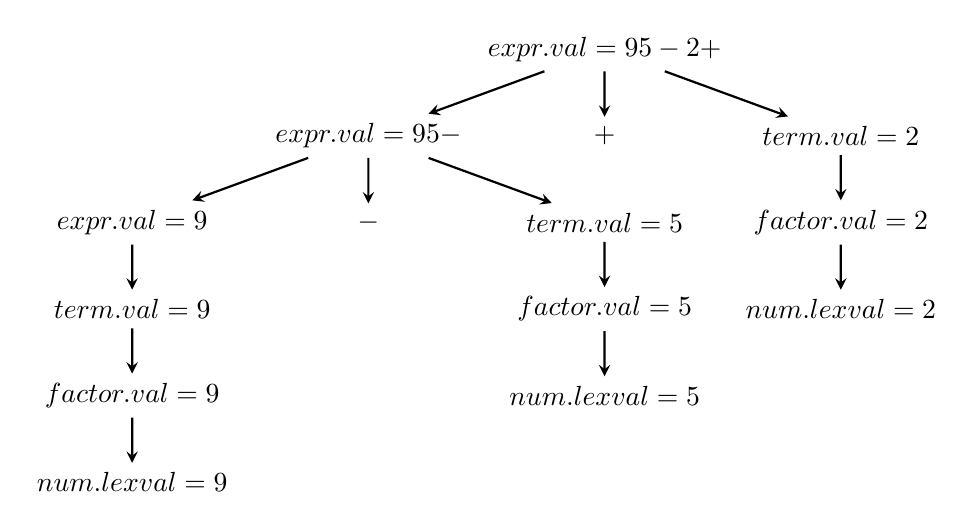
\begin{tikzpicture}[
    level distance=1.1cm,
    sibling distance=3cm,
    edge from parent/.style={draw,->,>=stealth,thick},
    every node/.style={align=center}
]
% 主树
\node {$expr.val = 95-2+$}
    child { node {$expr.val = 95-$}
        child { node {$expr.val = 9$}
            child { node {$term.val = 9$}
                child { node {$factor.val = 9$}
                    child { node {$num.lexval = 9$} }
                } 
            }  
        }
        child { node {$-$} }
        child { node {$term.val = 5$}
            child { node {$factor.val = 5$}
                child { node {$num.lexval = 5$} }
            } 
        }
    }
    child { node {$+$} }
    child { node {$term.val = 2$}
        child { node {$factor.val = 2$}
            child { node {$num.lexval = 2$} }
        }
    };
\end{tikzpicture}

对于中缀表达式 $9-5*2$,使用所给语法制导翻译方案构建的注释分析树如下:

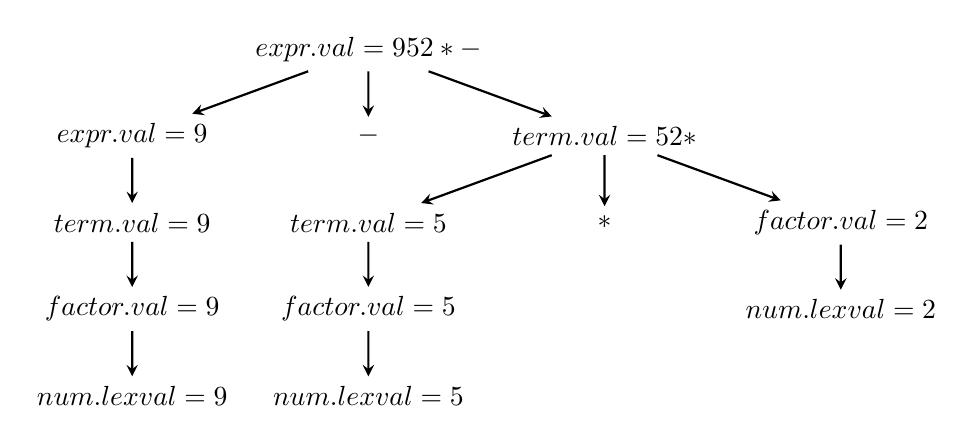
\begin{tikzpicture}[
  level distance=1.1cm,
  sibling distance=3cm,
  edge from parent/.style={draw,->,>=stealth,thick},
  every node/.style={align=center}
]
% 主树
\node {$expr.val = 952*-$}
  child { node {$expr.val = 9$}
      child { node {$term.val = 9$}
          child { node {$factor.val = 9$}
              child { node {$num.lexval = 9$} }
          } 
      }  
  }
  child { node {$-$} }
  child { node {$term.val = 52*$}
      child { node {$term.val = 5$}
          child { node {$factor.val = 5$}
              child { node {$num.lexval = 5$} }
          }
      }
      child { node {$*$} }
      child { node {$factor.val = 2$}
          child { node {$num.lexval = 2$} }
      } 
  };
\end{tikzpicture}

\noindent
\tbf{2.4}

在C语言中:

\begin{itemize}
  \item for语句开始时,创建一个新的作用域用于初始化子句
  \item 处理初始化子句中的声明并将标识符添加到这个新作用域
  \item 处理条件表达式
  \item 处理循环体之前,再创建一个新的嵌套作用域
  \item 处理循环体中的语句,将新声明的标识符添加到循环体作用域
  \item 处理更新表达式
  \item 循环体执行完后,退出循环体作用域
  \item for语句结束后,退出初始化子句作用域
\end{itemize}

在C++中:

\begin{itemize}
  \item for语句开始时,创建一个新的作用域
  \item 处理初始化子句中的声明并将标识符添加到此作用域
  \item 处理条件表达式
  \item 处理循环体中的语句,将新声明的标识符添加到同一个作用域(不允许重名)
  \item 处理更新表达式
  \item for语句结束后,退出此作用域
\end{itemize}

\noindent
\tbf{2.5}

所设计的文法如下:

\[
  \begin{array}{rcl}
    S & \to & 1 \\
    S & \to & 1D1 \\
    S & \to & 10D1 \\
    D & \to & 0 \\
    D & \to & 1 \\
    D & \to & 0D \\
    D & \to & 1D
  \end{array}
\]

\end{document}